\documentclass[11pt]{article}
% =====================================================================
%  CTX-anti (CTX-A) family --- the two program-feature categories.
%  Companion to i2s_anti_categories.tex / i2s_pro_categories.tex. Every
%  cited branch + value is REAL (from bench/dataset.jsonl, the per-branch
%  analysis cards, and the step5b_new_v3/ctx_coverage_LW arbiter
%  assignments). Compile: pdflatex ctx_anti_categories.tex
% =====================================================================
\usepackage[margin=1in]{geometry}
\usepackage{amsmath,amssymb}
\usepackage{xcolor}
\usepackage{listings}
\usepackage{booktabs}
\usepackage{tikz}
\usepackage{pgfplots}
\pgfplotsset{compat=1.16}
\usetikzlibrary{arrows.meta,positioning}

\definecolor{winc}{RGB}{30,120,60}   % winner (the flat-map arm that resolves) green
\definecolor{losc}{RGB}{190,60,60}   % loser  (the ctx arm that blocks) red
\definecolor{codebg}{RGB}{246,246,248}
\definecolor{kw}{RGB}{40,60,150}
\definecolor{cmt}{RGB}{120,120,120}
\definecolor{str}{RGB}{160,60,20}

\lstdefinestyle{c}{
  language=C, basicstyle=\ttfamily\small, backgroundcolor=\color{codebg},
  keywordstyle=\color{kw}\bfseries, commentstyle=\color{cmt}\itshape,
  stringstyle=\color{str}, numbers=none, frame=single, framerule=0pt,
  framesep=6pt, breaklines=true, showstringspaces=false, xleftmargin=4pt,
}

% tool / metric / rule / real-example box
\newcommand{\metricbox}[4]{%
  \par\smallskip\noindent\fbox{\parbox{\dimexpr\linewidth-2\fboxsep-2\fboxrule}{%
  \footnotesize
  \textbf{Tool:}~\texttt{#1}\\[2pt]
  \textbf{Metric:}~#2\\[2pt]
  \textbf{Verify rule (deterministic arbiter):}~\texttt{#3}\\[2pt]
  \textbf{Real example:}~#4}}\par\smallskip}

\title{\textbf{The CTX-anti family: two ways context-sensitive coverage backfires}}
\author{}
\date{}

\begin{document}
\maketitle
\vspace{-3em}

\paragraph{Backdrop.} \emph{CTX-anti} (CTX-A) collects the roadblocks where
\emph{context-sensitive coverage} \emph{hurts}: the plain coverage arm
(\emph{naive}) resolves the branch, but the same fuzzer with the call-context
hook (\emph{naive\_ctx}) blocks it. \texttt{CtxHook} folds a hash of the live
call-context (the caller chain) into every edge-map index, so the \emph{same}
control-flow edge counts as \emph{new} coverage under each distinct caller. That
extra dimension is exactly the I2S-anti story turned to feedback: the mechanism
meant to refine guidance instead \emph{inflates the coverage map}, and the
campaign spends its budget chasing context-redundant novelty instead of the
bytes the gate wants. The decisive pair is always the same ---
\emph{naive}$\,\succ\,$\emph{naive\_ctx} --- because adding only the context
dimension is the single-technique delta. Counts are validated roadblocks ($n$);
the family has $n=4$ validated in \emph{one} category with two measurement
routes, plus a residual shallow-literal tail (\S2) that is honestly
\emph{inconclusive}.

\smallskip\noindent\textit{A note on the signal.} Context-sensitive coverage is
a \emph{non-local feedback} (like value-profile): it leaves no event in any
single seed's mutation lineage. The only handles are what the two corpora
\emph{reach} or \emph{hoard}. The one validated category has \emph{two
measurement routes} for the same backfire, depending on which handle fires:
corpus \emph{size} (the ctx arm hoards a bloated corpus, route~A) or per-seed
\emph{depth} (the flat arm drives the gate deeper while the ctx arm fragments and
stalls, route~B). Figure~\ref{fig:ctx-anti} shows both side by side.

% =====================================================================
\section*{1.\ \ The context dimension inflates coverage redundantly \hfill {\normalsize\texttt{ctx\_inflation} ($n=4$)}}
Context-sensitive coverage makes the \emph{same} control flow look novel under
each call-context, so \emph{naive\_ctx} spends the campaign chasing
context-redundant ``new'' coverage instead of the bytes the gate wants. This
backfire surfaces through \textbf{two measurement routes} --- the ctx arm hoards
a bloated \emph{corpus} (route~A), or it fragments a deep path so no seed reaches
the gate \emph{depth} the branch needs (route~B). Same anti-mechanism (redundant
context inflation), two handles; which fires is a property of the gate. (We
earlier split these as two categories --- \emph{ctx\_corpus\_inflation} ($2$) and
\emph{ctx\_depth\_inflation} ($2$) --- but they are one mechanism with two routes,
merged 2026-06-26.)

\paragraph{Route A --- corpus bloat (\texttt{corpus\_count\_ratio}).} A deep,
repeatedly-entered code path makes the \emph{same} edges look novel once
per call-context, so \emph{naive\_ctx} hoards far more (context-redundant) corpus
entries than \emph{naive}. The bloated corpus spreads the mutation budget thin
--- the fuzzer is busy re-saving the same control flow under fresh context
hashes instead of mutating the bytes that flip the gate.

\begin{lstlisting}[style=c]
// libpng  pngrutil.c : png_read_IDAT_data()
} while (ret != Z_STREAM_END);          // deep inflate do/while loop
if (png_ptr->zstream.avail_in > 0 ||    // <-- blocker (libpng/4072):
    png_ptr->idat_size > 0)             //     residual IDAT bytes left over
\end{lstlisting}

\noindent The branch needs residual compressed bytes after zlib returns
\texttt{Z\_STREAM\_END}. \emph{naive} flips it with ordinary havoc; but the deep
inflate loop is re-entered \emph{2750} times per loser seed (vs \emph{136} per
winner), and \texttt{naive\_ctx} folds a context hash into each iteration's
edges, so every revisit looks like new coverage. It hoards a corpus
$3.7\times$ larger than naive's and never spends the budget on the byte-level
mutation that manufactures the extra-data condition.

\metricbox{corpus\_queue (saved-corpus count, per trial)}
{\texttt{corpus\_count\_ratio} $=$ median(saved entries, \emph{naive\_ctx}) $/$ median(saved entries, \emph{naive})}
{winner $=$ naive\_ctx AND corpus\_count\_ratio $\ge 1.5$}
{libpng/4072 (\texttt{png\_read\_IDAT\_data:4245}) --- \texttt{naive\_ctx} saves \emph{16{,}761} entries vs naive's \emph{4{,}500}: \texttt{corpus\_count\_ratio}$=3.73$. lcms/2149 (\texttt{\_cmsReadHeader:776}, the 128-byte-header underflow gate) shows the same sign at \emph{1095} vs \emph{636}: \texttt{corpus\_count\_ratio}$=1.72$.}

% per-category plot consolidated into Fig.~\ref{fig:ctx-anti} (after section 2)

% =====================================================================
\paragraph{Route B --- depth fragmentation (\texttt{depth\_lift}).} Here the gate
sits at the bottom of a tight, deeply-iterated path (a scan loop or
a wide \texttt{switch}). \emph{naive}'s flat per-edge map lets a single seed drive
the path \emph{deep} and converge on the exact operand; \texttt{naive\_ctx}
shatters that path's edges across call-context slots, diluting the feedback so no
seed reaches the gate depth the branch needs. The fingerprint is a per-seed
\emph{depth lift} on the resolving arm: the winner reaches the gate far deeper
than the ctx loser ever does.

\begin{lstlisting}[style=c]
// libxml2  parser.c : xmlParseCharData()
do {                                 // tight char-data scan loop
    ...
    if (*in == 0xD) { ... continue; }   // CR handler keeps the loop alive
} while (IS_CHAR(*in));              // <-- blocker (libxml2/6576:4610)
\end{lstlisting}

\noindent The gate needs a long char-data run with embedded CR/LF that keeps the
\texttt{do}-\texttt{while} alive. \emph{naive} assembles 1862-byte bodies that
loop deep (per-seed depth \emph{97.5}); \texttt{naive\_ctx}'s context-split edges
dilute the scan-loop signal so its seeds stall shallow (\emph{22.2}) and the loop
falls through to \texttt{xmlParseCharDataComplex}, leaving the true side blocked.

\metricbox{depth\_reach (\texttt{bench/tools/depth\_reach.py})}
{\texttt{depth\_lift} $=$ winner\_depth $/$ loser\_depth (per-seed reach at the blocker line, \emph{naive} vs \emph{naive\_ctx}); \texttt{winner\_deeper}}
{depth\_lift $\ge 2.0$ AND winner\_deeper $==$ True}
{libxml2/6576 (\texttt{xmlParseCharData:4610}) --- winner\_depth \emph{97.5} vs loser\_depth \emph{22.2}: \texttt{depth\_lift}$=4.39$. harfbuzz/6124 (\texttt{\_hb\_preprocess\_text\_vowel\_constraints:409}, the Tirhuta \texttt{case 0x1148Bu/0x1148Du}) --- naive converges on the exact codepoint (depth \emph{2.0}) while the ctx arm disperses across sibling Tirhuta cases (depth \emph{0.1}): \texttt{depth\_lift}$=4.0$.}

\begin{figure}[t]
\centering
% ---- panel 1: corpus_inflation ----
\begin{minipage}[b]{0.46\linewidth}\centering
\resizebox{\linewidth}{!}{%
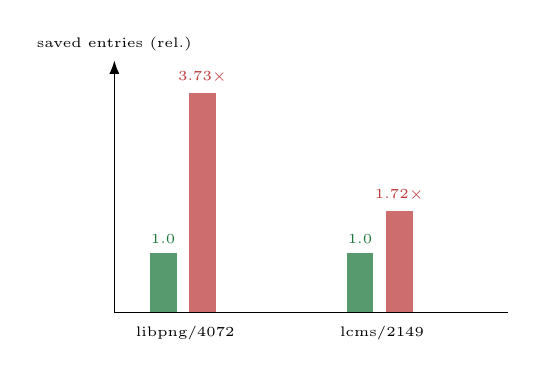
\begin{tikzpicture}[font=\scriptsize,>=Latex]
  \def\bw{0.34}
  \draw[->] (0,0)--(0,3.2) node[above,font=\tiny]{saved entries (rel.)};
  \draw (0,0)--(5.0,0);
  % libpng: naive 4500 -> 1.0, naive_ctx 16761 -> 3.725  (scale 0.75/unit)
  \fill[winc!75] (0.45,0) rectangle ++(\bw,0.75);
  \node[font=\tiny,winc,above] at (0.62,0.75) {1.0};
  \fill[losc!75] (0.95,0) rectangle ++(\bw,2.79);
  \node[font=\tiny,losc,above] at (1.12,2.79) {3.73$\times$};
  \node[font=\tiny,below] at (0.9,-0.05) {libpng/4072};
  % lcms: naive 636 -> 1.0, naive_ctx 1095 -> 1.722
  \fill[winc!75] (2.95,0) rectangle ++(\bw,0.75);
  \node[font=\tiny,winc,above] at (3.12,0.75) {1.0};
  \fill[losc!75] (3.45,0) rectangle ++(\bw,1.29);
  \node[font=\tiny,losc,above] at (3.62,1.29) {1.72$\times$};
  \node[font=\tiny,below] at (3.4,-0.05) {lcms/2149};
\end{tikzpicture}}\\[2pt]
{\scriptsize\textbf{route A: corpus}}\\{\tiny ctx arm \emph{hoards} a bloated corpus}
\end{minipage}\hfill
% ---- panel 2: depth_inflation ----
\begin{minipage}[b]{0.46\linewidth}\centering
\resizebox{\linewidth}{!}{%
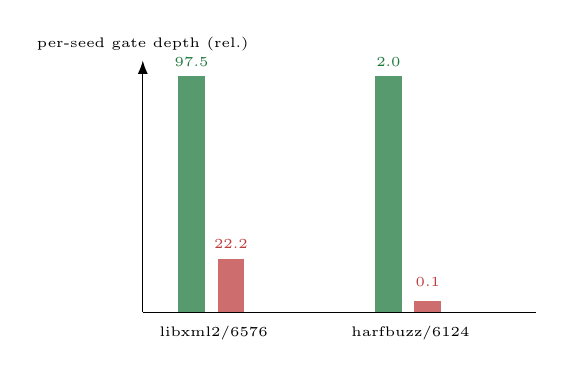
\begin{tikzpicture}[font=\scriptsize,>=Latex]
  \def\bw{0.34}
  \draw[->] (0,0)--(0,3.2) node[above,font=\tiny]{per-seed gate depth (rel.)};
  \draw (0,0)--(5.0,0);
  % libxml2: naive 97.5 -> 3.0, naive_ctx 22.2 -> 0.683 (scale: 97.5->3.0)
  \fill[winc!75] (0.45,0) rectangle ++(\bw,3.0);
  \node[font=\tiny,winc,above] at (0.62,3.0) {97.5};
  \fill[losc!75] (0.95,0) rectangle ++(\bw,0.683);
  \node[font=\tiny,losc,above] at (1.12,0.683) {22.2};
  \node[font=\tiny,below] at (0.9,-0.05) {libxml2/6576};
  % harfbuzz: naive 2.0, naive_ctx 0.1  (scale 2.0 -> 3.0)
  \fill[winc!75] (2.95,0) rectangle ++(\bw,3.0);
  \node[font=\tiny,winc,above] at (3.12,3.0) {2.0};
  \fill[losc!75] (3.45,0) rectangle ++(\bw,0.15);
  \node[font=\tiny,losc,above] at (3.62,0.20) {0.1};
  \node[font=\tiny,below] at (3.4,-0.05) {harfbuzz/6124};
\end{tikzpicture}}\\[2pt]
{\scriptsize\textbf{route B: depth}}\\{\tiny flat arm reaches the gate \emph{deeper}}
\end{minipage}
\caption{The two routes of \texttt{ctx\_inflation}. \textbf{Left (route A):} corpus
bloat --- the context arm (\emph{naive\_ctx}, red) hoards a corpus $\ge1.5\times$ larger
than the flat arm (\emph{naive}, green), because the same edges look novel under
each call-context; bars are normalized to naive$\,{=}\,1$. \textbf{Right (route B):}
depth fragmentation --- the flat arm (green) drives the gate far deeper
per seed than the context arm (red), which fragments the deep path across context
slots; bars are absolute per-seed reach at the blocker line. In both, the arm with
the \emph{context} dimension is the one that blocks.}
\label{fig:ctx-anti}
\end{figure}

% =====================================================================
\section*{2.\ \ The residual tail: shallow-literal dilution \hfill {\normalsize\emph{inconclusive} ($n=2$)}}
Two members --- libxml2/6605 (\texttt{name[1]=='m'/'M'}) and harfbuzz/5802 (the
paired SHIN+SIN-DOT codepoint) --- are \emph{shallow} exact-literal equality
gates. The mechanism story is plausible (\texttt{naive\_ctx} splits the per-edge
reward across context slots so the winning literal is never assembled), but it is
\emph{not discriminable} by any built corpus measurement. Because ctx is a
non-local feedback whose footprint a shallow 1-hop gate's corpus does not
preserve, all four permitted handles were scored across the labeling rounds and
\emph{none} held: corpus \emph{size} (\texttt{corpus\_size\_ratio}$<1.5$),
call-\emph{depth} (\texttt{call\_count\_lift}$\sim1$, no loop to flood),
fixed-offset \emph{byte presence} (\texttt{signed\_target\_enrich} did not reach
$\le-0.5$), and offset-tolerant \emph{window distance}
(\texttt{value\_distance\_reached}: no sustained approach gap). The remaining
built tools (\texttt{joint\_necessity}, \texttt{token\_count}) measure structural
\emph{assembly} for a different (vpc-vs-cmplog) subtype and do not fit a
single-byte equality gate. Per guardrail G3, an honest \emph{inconclusive} is the
correct outcome here, not a forced label.

% =====================================================================
\section*{At a glance}
\begin{center}\small
\begin{tabular}{@{}p{3.2cm}clp{5.0cm}@{}}
\toprule
\textbf{Category} & \textbf{$n$} & \textbf{Example} & \textbf{How the context dimension backfires} \\
\midrule
ctx\_inflation & 4 & libpng/4072 (A), libxml2/6576 (B) & \textbf{route A} deep re-entered path $\Rightarrow$ same edges look novel per context $\Rightarrow$ ctx arm hoards a bloated corpus (\texttt{corpus\_count\_ratio}$\ge1.5$); \textbf{route B} tight deep loop / wide switch $\Rightarrow$ ctx fragments the path $\Rightarrow$ flat arm reaches the gate deeper (\texttt{depth\_lift}$\ge2.0$) \\
\midrule
\emph{(shallow-literal dilution)} & 2 & libxml2/6605 & non-local feedback, no corpus footprint at a 1-hop gate $\Rightarrow$ honestly \emph{inconclusive} (G3) \\
\midrule
\textbf{CTX-A validated} & \textbf{4} & & decisive pair \emph{naive}$\,\succ\,$\emph{naive\_ctx} throughout \\
\bottomrule
\end{tabular}
\end{center}

\noindent\footnotesize All counts and metric values are from
\texttt{bench/dataset.jsonl}, the per-branch analysis cards, and the
\texttt{step5b\_new\_v3/ctx\_coverage\_LW} arbiter assignments; the verify rules
are the deterministic arbiter rules (no LLM in the decision). lcms/2149 and
libpng/4072 are corpus targets on server~sB; harfbuzz/6124 on s4; libxml2/6576 on
sB --- each scored by its owning server.
\end{document}
